\section{Взаимное влияние процессов четырёхволнового смешения в оптических волокнах}

\begin{frame}
	\frametitle{Взаимное влияние процессов четырёхволнового смешения в оптических волокнах}
	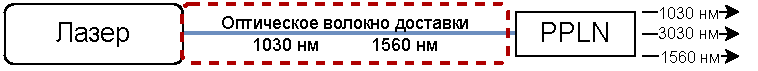
\includegraphics[width=\linewidth]{Presentation/images/problem_fiber}
	\fixme{Мотивация, задача}
	\begin{columns}[t]
		\begin{column}{0.49\textwidth}
			\fixme{хз}
		\end{column}
		\begin{column}{0.49\textwidth}
			\fixme{что говорить. мб ограничения мощи или длині волокна...}
		\end{column}
	\end{columns}
\end{frame}

\begin{frame}
	\frametitle{Взаимное влияние процессов четырёхволнового смешения в оптических волокнах}

	
	\begin{center}
		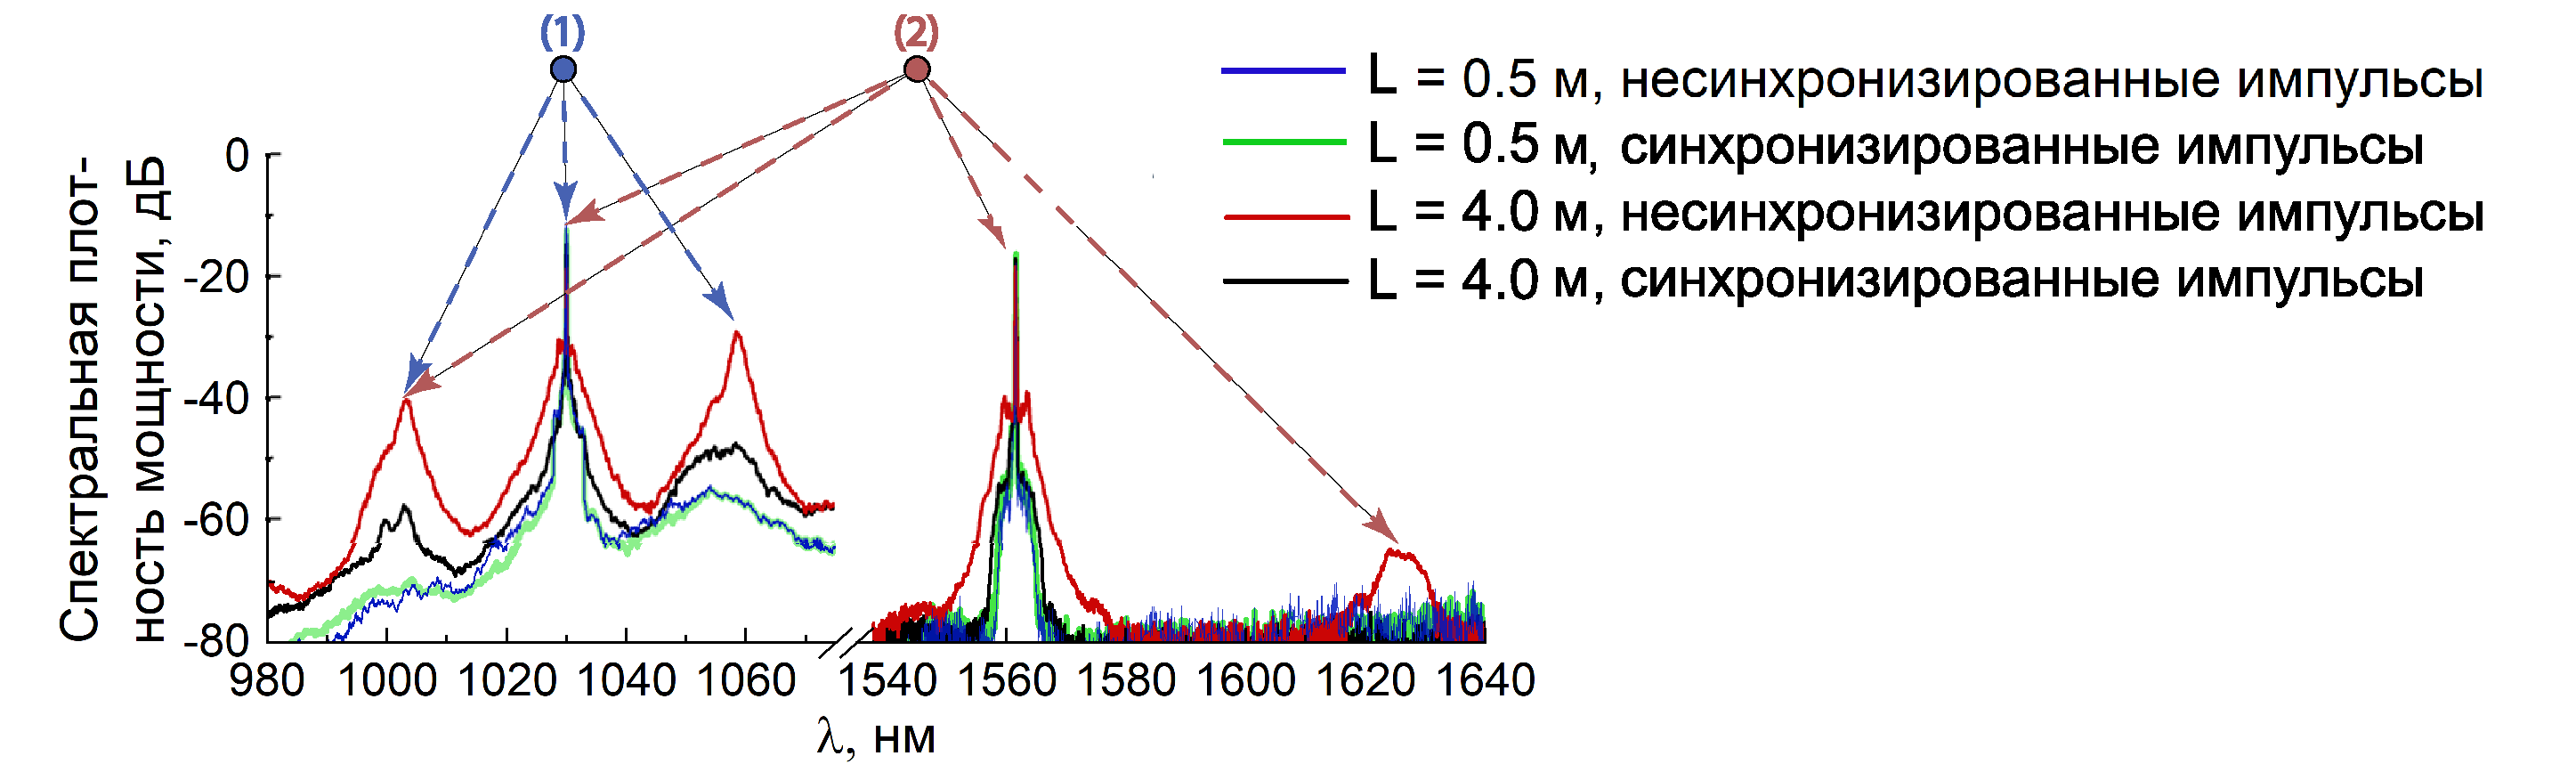
\includegraphics[width=0.85\linewidth]{Dissertation/images/imfwm/problem_2conf_1}
		
		\footnotesize{Измеренные спектры двухволнового лазера. $L$: длина ОВ}
		
		\begin{columns}
			\begin{column}{0.76\textwidth}			
				\begin{align*}
					\text{ММ ЧВС:}~\LPoi^{1030}+\LPii^{1030}&\longrightarrow \LPoi^{1003}+\LPii^{1059}\\
					\text{ОМ ЧВС:}~\LPoi^{1030}+\LPoi^{1562}&\longrightarrow \LPoi^{1003}+\LPoi^{1629}	
				\end{align*}			
			\end{column}
			\begin{column}{0.24\textwidth}
				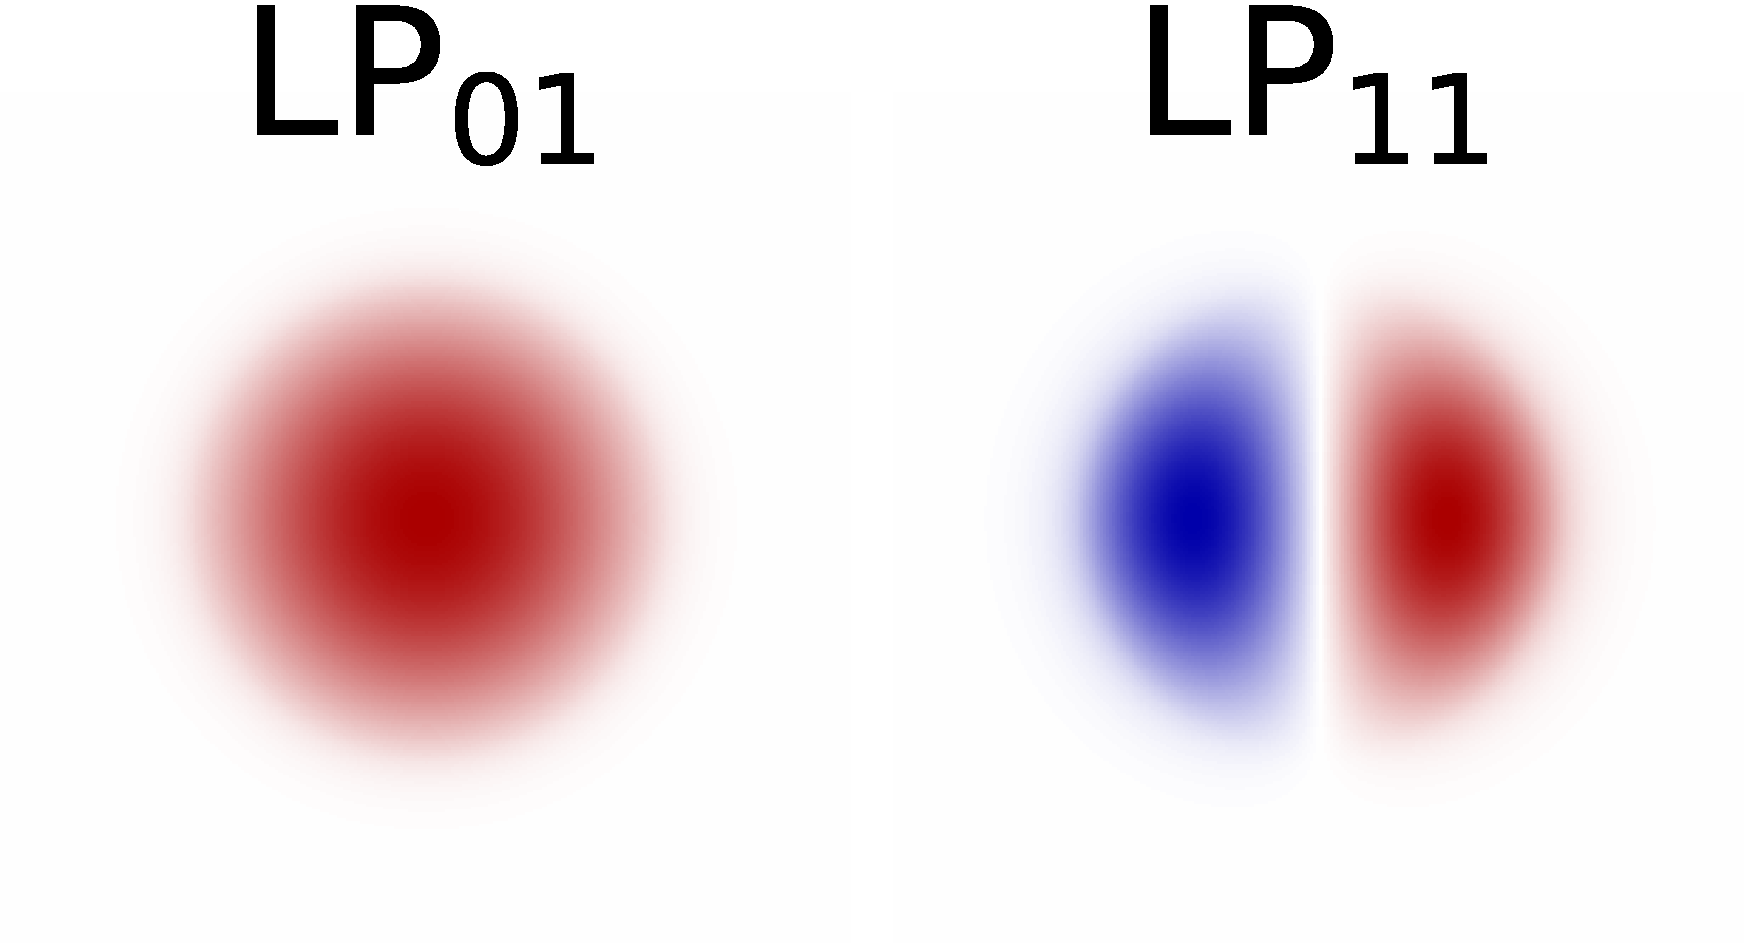
\includegraphics[width=0.7\linewidth]{Dissertation/images/review/lp_modes_01_11_preza.pdf}
			\end{column}
		\end{columns}
	\end{center}
	\hfill
	
	\footnotesize
	Проверка:
	
	\begin{itemize}
		\item Спектр при известном модовом составе;
		\item Модовый состав при известном спектре;
		\item Численный расчёт
	\end{itemize}	
\end{frame}

\begin{frame}
	\frametitle{Взаимное влияние процессов четырёхволнового смешения в оптических волокнах}
	\framesubtitle{Математическая модель ЧВС}

	\begin{columns}
		\begin{column}{0.48\textwidth}
			\scalebox{0.7}{%
			\begin{minipage}{\textwidth}
				\begin{equation*}
					\left\{\begin{array}{@{}l@{}}
						\dfrac{dA_1}{dz}=\dfrac{\im n_{nl} \omega_1}{c}\!\left[\left(f_{11}\left|A_1\right|^2+\sum\limits_{k\neq1}f_{1k}\left|A_k\right|^2\right)\!A_1+2f_{1234}A_2^{\ast}A_3A_4\e^{\im \Delta k z}\right]\!, \vspace{0.05cm} \\ 
						\dfrac{dA_2}{dz}=\dfrac{\im n_{nl} \omega_2}{c}\!\left[\left(f_{22}\left|A_2\right|^2+\sum\limits_{k\neq2}f_{2k}\left|A_k\right|^2\right)\!A_2+2f_{2134}A_1^{\ast}A_3A_4\e^{\im \Delta k z}\right], \vspace{0.05cm} \\
						\dfrac{dA_3}{dz}=\dfrac{\im n_{nl} \omega_3}{c}\!\left[\left(f_{33}\left|A_3\right|^2+\sum\limits_{k\neq3}f_{3k}\left|A_k\right|^2\right)\!A_3+2f_{3412}A_4^{\ast}A_2A_1\e^{-\im \Delta k z}\right], \vspace{0.05cm} \\
						\dfrac{dA_4}{dz}=\dfrac{\im n_{nl} \omega_4}{c}\!\left[\left(f_{44}\left|A_4\right|^2+\sum\limits_{k\neq4}f_{4k}\left|A_k\right|^2\right)\!A_4+2f_{4312}A_3^{\ast}A_2A_1\e^{-\im \Delta k z}\right].
					\end{array}\right.\,	
					\label{eq:mainEQfwm}
				\end{equation*}
			\end{minipage}
		}
		\end{column}
		\begin{column}{0.52\textwidth}
			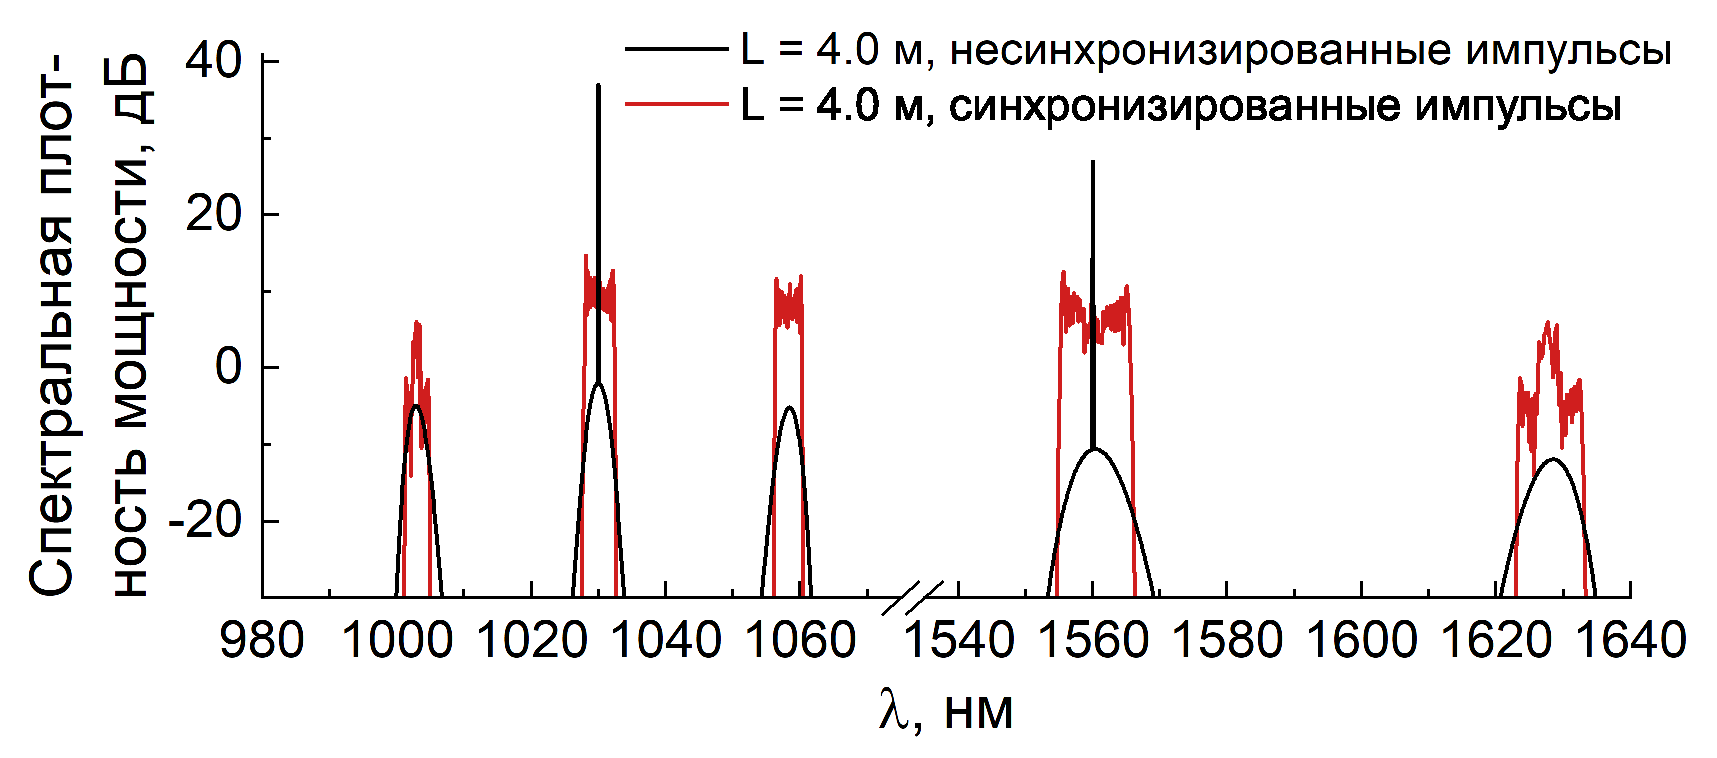
\includegraphics[width=\linewidth]{Dissertation/images/imfwm/model_spectra.eps}
			
			\centering
			\footnotesize{
			Рассчитанные спектры двухволнового лазера для несинхронизированных (чёрный) и синхронизированных (красный) импульсов}
		\end{column}
	\end{columns}
	
	\vfill
	\footnotesize{$A_{{i}}$~--- амплитуды взаимодействующих волн с циклическими частотами $\omega_i$; $n_{nl}$~--- нелинейный показатель преломления; $f_{ij}\text{ и }f_{ijkl}$ $\left(i,j,k,l\in\left[1,\,4\right]\right)$~--- интегралы перекрытия между поперечными модами ОВ и их парами соответственно; $z$~--- продольная координата; $\Delta k$~--- волновая расстройка, ${n_{i}}$~--- эффективный модовый показатель преломления, $c$~--- скорость света в вакууме.}
\end{frame}


\begin{frame}
	\frametitle{Взаимное влияние процессов четырёхволнового смешения в оптических волокнах}
	\framesubtitle{Подавление ММ ЧВС}
	
	\begin{columns}
		\begin{column}{0.5\textwidth}
			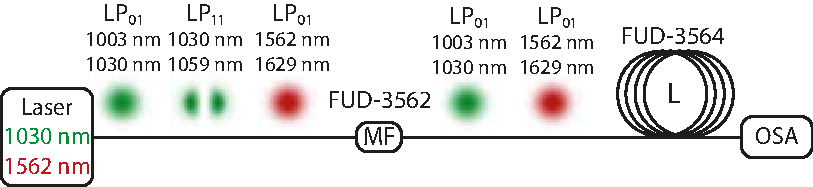
\includegraphics[width=\linewidth]{Dissertation/images/imfwm/scheme_suppression}
			\footnotesize{Экспериментальная установка для подавления ММЧВС. MF: модовый фильтр, OSA: оптический спектроанализатор}
		\end{column}
		\begin{column}{0.5\textwidth}
			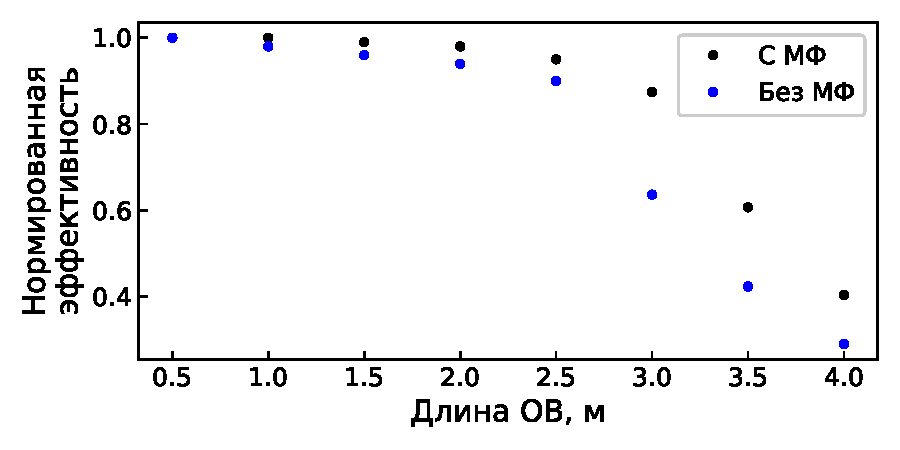
\includegraphics[width=\linewidth]{Dissertation/images/imfwm/dfg_eff_mf.pdf}
			
			\centering
			\footnotesize{
				Зависимость нормированной эффективности ГРЧ от длины ОВ при использовании МФ на входе ОВ (чёрные точки), без использования МФ (синие точки)}
		\end{column}
	\end{columns}
	
\end{frame}


\begin{frame}
	\frametitle{Взаимное влияние процессов четырёхволнового смешения в оптических волокнах}
	\framesubtitle{Положение, выносимое на защиту}
	
	В маломодовом оптическом волокне взаимное влияние одномодового и межмодового четырёхволнового смешения синхронизированных оптических импульсов двухволнового лазерного источника обусловлено перекрытием спектров усиления их общих антистоксовых компонент.
	
	
\end{frame}